
\chapter{Hynesim installation}

\section{Hynesim}



\section{Import of virtual machines}

Hynesim works with many virtual software as qemu, virtualbox, and vmware. For this project I use qemu because it is
the most suitable for hynesim. To create virtual computer on hynesim, I firstly created the machine on virtualbox,
then I converted it to a qemu virtual machine and to finish I import this machine to hynesim.

Hynesim is also provided with some virtual equipment: a switch, and an inter topology link.

An important detail, on the hynesim network machines haven't access to the internet. So I had to do update, and
install before they are imported.

I created the left part of the network represented on the figure \ref{fig:network}.


\begin{figure}[h]
  \centering
  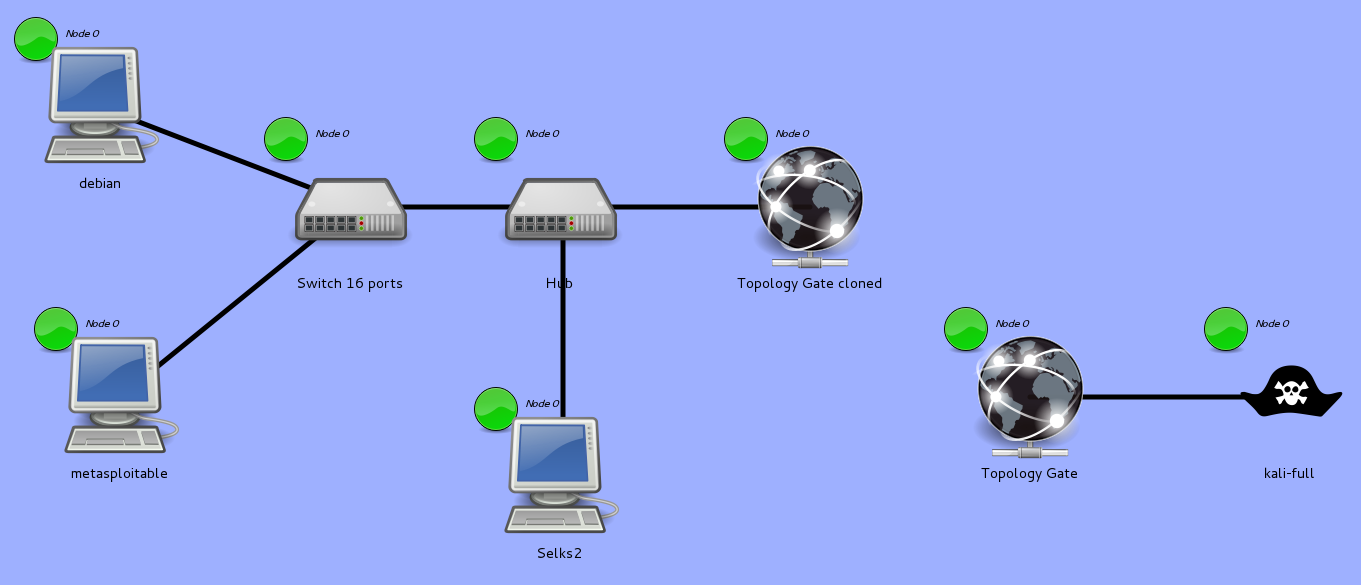
\includegraphics[width=\textwidth]{network_infra}
  \caption{Network infrastructure}
  \label{fig:network}
\end{figure}

\section{Selks}

As it was explain on the previous section, before importing the machine I had to create an virtual machine. To do
so, I use an ISO available on the Stamus web page \cite{stamusnetworks:_selks} and I create a virtual machine with
it. Then, before it was imported, I have set up important libraries for the realization of the SIEM\footnote{More
  information on the chapter \ref{sec:SIEM}}.

The ISO is a key in hand version. So Suricata, Elasticsearch, Logstash, Kibana, Scirius, and Evebox are already
installed and connected. However, I had to configure some particularity and take in charge the system.

The only particularity that I have to configure during the installation was the network. In fact, on the hynesim
network there is no DHCP, so I had to configure by hand the IP of the machines. Moreover, I had to configure on
Suricata the private address domain. In fact, Suricata doesn't pay so much attention to networks packets from the
private network.

Then, I tested my IDS with basic attacks\footnote{These attacks were achieve by Justin Bouroux}. The can see on the
figure \ref{fig:evebox} the evebox interface which permit to visualize alerts raised by Suricata.

\begin{figure}[h]
  \centering
  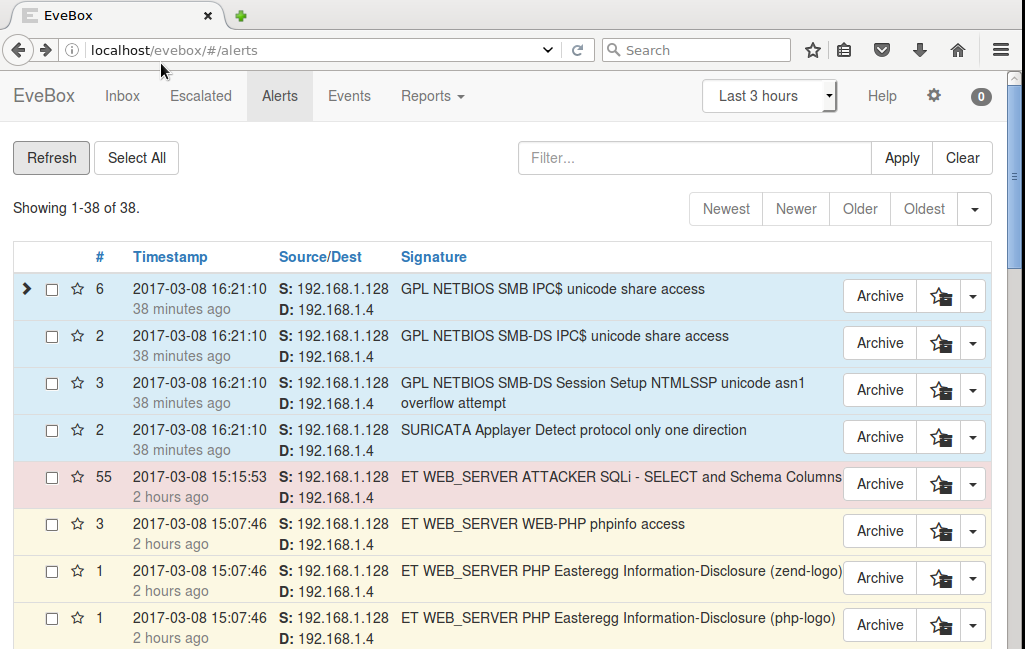
\includegraphics[width=\textwidth]{evebox}
  \caption{Example of alerts}
  \label{fig:evebox}
\end{figure}


%%% Local Variables:
%%% mode: latex
%%% TeX-master: "../rapport_de_base"
%%% End:
